\documentclass[11pt]{article}

\usepackage[a4paper,margin=1in]{geometry}
\usepackage{amsmath,amssymb,bm}
\usepackage{booktabs,tabularx}
\usepackage{tikz}
\usetikzlibrary{arrows.meta,positioning}
\usepackage[hidelinks]{hyperref}

\newcommand{\E}{\mathbb{E}}
\newcommand{\dd}{\mathop{}\!\mathrm{d}}
\newcommand{\KL}{D_{\mathrm{KL}}}
\newcolumntype{Y}{>{\raggedright\arraybackslash}X}

\title{Reinforcement Learning for LLM Fine-Tuning\\
from the Path-Integral Perspective}
\author{}
\date{}

\begin{document}

\maketitle
\tableofcontents

\newpage
\section{Introduction}

\subsection{Some basic definitions}

We first identify the objects involved in reinforcement learning.

\begin{enumerate}
    \item The state at time \(t\) is \(S_t\).

    \item The action at time \(t\) is \(a_t\).  It labels the transition
    from \(S_t\) to \(S_{t+1}\), whose probability is
    \(P(S_{t+1}\mid S_t,a_t)\).

    \item A stationary policy \(\pi\) is a global rule that assigns a
    distribution of actions to each state.  Associate the action \(a_t\)
    with the operator \(\hat a_t\).  Then
\end{enumerate}

\begin{equation}
    \begin{split}
    \hat\pi|S_t\rangle
    &=\int da_t\;\pi(a_t\mid S_t)\hat a_t|S_t\rangle\\
    &\equiv\hat\pi(S_t)|S_t\rangle,
    \end{split}
    \label{eq:policy-operator}
\end{equation}

where
\(\hat\pi(S_t)=\int da_t\,\pi(a_t\mid S_t)\hat a_t\).
For a discrete action space, the integral is replaced by a sum.

Let \(\pi_\theta\) denote a policy parameterized by \(\theta\).  For the
trajectory

\begin{equation}
    \begin{split}
        T=(S_0,a_0,S_1,a_1,\ldots,a_{N-1},S_N),
    \end{split}
    \label{eq:trajectory}
\end{equation}

where \(N\) is the number of transitions, the probability induced by
\(\pi_\theta\) is

\begin{equation}
    \begin{split}
    P(T\mid\pi_\theta)=\rho(S_0)\prod_{i=0}^{N-1}
    P(S_{i+1}\mid S_i,a_i)\pi_\theta(a_i\mid S_i),
    \end{split}
    \label{eq:path-measure}
\end{equation}

where \(\rho(S_0)\) is the initial-state distribution.  This is the path
measure.

\subsection{Reward and return}

The reward at step \(i\) is

\begin{equation}
    \begin{split}
        r_i=R(a_i,S_i,S_{i+1}),
    \end{split}
    \label{eq:reward}
\end{equation}

Let \(0\leq\gamma\leq1\) be the discount factor.  The total return along
\(T\) is

\begin{equation}
    \begin{split}
        G_0[T]=\sum_{i=0}^{N-1}\gamma^i r_i.
    \end{split}
    \label{eq:return}
\end{equation}

The return remaining from time \(t\) is

\begin{equation}
    \begin{split}
        G_t=\sum_{i=t}^{N-1}\gamma^{i-t}r_i.
    \end{split}
    \label{eq:return-to-go}
\end{equation}

The expected return is

\begin{equation}
    \begin{split}
        J(\theta)=\int \mathcal D S\,\mathcal D a\;
        P(T\mid\pi_\theta)G_0[T]
        =\left\langle G_0[T]\right\rangle_{T\sim\pi_\theta}.
    \end{split}
    \label{eq:expected-return}
\end{equation}

Here \(\mathcal D S\,\mathcal D a\) denotes the sum or integral over all
state--action paths.

Fixing the initial state gives the on-policy value function,

\begin{equation}
    \begin{split}
        V^\pi(S)=\left\langle G_0[T]\right\rangle_{T\sim\pi;\,S_0=S}.
    \end{split}
    \label{eq:value}
\end{equation}

The word ``initial'' refers to the path segment being averaged.  At time
\(t\), the current state \(S_t\) is the initial state of the remaining path,
so

\begin{equation}
    \begin{split}
        V^\pi(S_t)=\E\left[G_t\mid S_t\right].
    \end{split}
    \label{eq:value-current-state}
\end{equation}

Fixing the initial state and action gives the \(Q\) function,

\begin{equation}
    \begin{split}
        Q^\pi(S,a)=\left\langle G_0[T]\right\rangle_{T\sim\pi;\,S_0=S,a_0=a}.
    \end{split}
    \label{eq:action-value}
\end{equation}

Averaging over the first action recovers the value function:

\begin{equation}
    \begin{split}
        V^\pi(S)=\int\dd a\;\pi(a\mid S)Q^\pi(S,a).
    \end{split}
    \label{eq:value-from-action-value}
\end{equation}

At time \(t\), their difference is the advantage,

\begin{equation}
    \begin{split}
        A^\pi(S_t,a_t)=Q^\pi(S_t,a_t)-V^\pi(S_t).
    \end{split}
    \label{eq:advantage}
\end{equation}

\subsection{Policy gradient}

The optimal policy maximizes the expected return.  At an interior optimum,

\begin{equation}
    \begin{split}
        \nabla_\theta J(\theta)=0.
    \end{split}
    \label{eq:stationary-policy}
\end{equation}

Assume that the reward function has no explicit \(\theta\) dependence, so
\(G_0[T]\) is fixed when a path is fixed.  Using

\begin{equation}
    \begin{split}
        \nabla_\theta\pi_\theta(a_t\mid S_t)
        =\pi_\theta(a_t\mid S_t)\nabla_\theta\log\pi_\theta(a_t\mid S_t)
    \end{split}
    \label{eq:log-derivative}
\end{equation}

gives

\begin{equation}
    \begin{split}
        \nabla_\theta J(\theta)
        =\left\langle G_0[T]\nabla_\theta
        \log P(T\mid\pi_\theta)\right\rangle.
    \end{split}
    \label{eq:policy-gradient-path}
\end{equation}

When \(\rho\) and \(P\) do not depend on \(\theta\),

\begin{equation}
    \begin{split}
        \nabla_\theta\log P(T\mid\pi_\theta)
        =\sum_{i=0}^{N-1}\nabla_\theta\log\pi_\theta(a_i\mid S_i).
    \end{split}
    \label{eq:path-score}
\end{equation}

The corresponding surrogate loss is

\begin{equation}
    \begin{split}
        \mathcal L_{\mathrm{PG}}(\theta)
        =-\widehat{\E}\left[
        G_0[T]\sum_{i=0}^{N-1}
        \log\pi_\theta(a_i\mid S_i)\right].
    \end{split}
    \label{eq:policy-gradient-surrogate}
\end{equation}

Here \(\widehat{\E}\) is the average over sampled paths.  Their returns are
held fixed while differentiating the loss.  The first derivative of
Eq.~\eqref{eq:policy-gradient-surrogate} gives the sampled policy gradient;
the surrogate and \(-J\) are not the same function and need not have the same
higher derivatives.

\newpage
\section{The LLM Post-Training Problem}

An LLM already defines a distribution over responses.  For a prompt \(x\)
and a response \(y=(y_1,\ldots,y_L)\), identify

\begin{equation}
    \begin{split}
        S_t=(x,y_{<t}),
        \qquad
        a_t=y_t,
        \qquad
        S_{t+1}=(x,y_{\leq t}).
    \end{split}
    \label{eq:llm-state-action}
\end{equation}

Here \(\pi_\theta(\cdot\mid S_t)\) is the next-token distribution produced
by the complete LLM.  The action space is the vocabulary, and a complete
response is a path of token actions.  Which network parameters are included
in \(\theta\) is a separate implementation choice.  Appending \(y_t\) is a
deterministic transition, so for the complete path \(T=(x,y)\),

\begin{equation}
    \begin{split}
        P(T\mid\pi_\theta)
          =q(x)\prod_{t=1}^{L}
           \pi_\theta(y_t\mid x,y_{<t}),
    \end{split}
    \label{eq:autoregressive-path}
\end{equation}

where \(q\) is the prompt distribution and \(q(x)\) is its probability mass
or density.  The LLM supplies the policy and
therefore the path measure.  The post-training problem is to move probability
mass toward paths that exhibit reasoning.

Let \(\mathcal C_x\) be the set of responses that pass a specified reasoning
criterion for prompt \(x\).  If this criterion can be evaluated exactly, then

\begin{equation}
    \begin{split}
        P_\theta(\mathcal C)
          =\E_{x\sim q}\left[
           \sum_{y\in\mathcal C_x}\pi_\theta(y\mid x)
           \right].
    \end{split}
    \label{eq:reasoning-probability}
\end{equation}

Thus increasing reasoning capability means increasing the probability mass
in \(\mathcal C_x\).  More generally, training uses a measurable sequence
score \(\mathcal R(x,y)\), supplied by a verifier, human preference, or
learned reward model.  It is treated as the complete-path return.  Unless
stated otherwise, LLM training in this note uses the undiscounted return
\(\gamma=1\).  From this point onward, \(\gamma\) is therefore suppressed.

Section~1 indexed generic transitions from zero.  Here tokens are indexed by
\(t=1,\ldots,L\).  The one-step reward \(r_t\) is assigned after \(y_t\)
extends \(S_t\).  Since \(S_{t+1}\) is determined by \(S_t\) and \(y_t\),
write

\begin{equation}
    \begin{split}
        r_t&=R(S_t,y_t),\\
        G_t&=\sum_{i=t}^{L}r_i.
    \end{split}
    \label{eq:llm-token-reward}
\end{equation}

Here \(L\) is the response length.  If the score is assigned only after the
last token, then \(r_t=\Theta(t-L)\mathcal R(x,y)\), where
\(\Theta(t-L)=0\) for \(t<L\) and \(\Theta(0)=1\).  This gives
\(G_1=\mathcal R(x,y)\).  The value, action-value, and advantage functions
become

\begin{equation}
    \begin{split}
        V^\pi(S_t)
          &=\E\left[G_t\mid S_t\right],\\
        Q^\pi(S_t,y_t)
          &=\E\left[G_t\mid S_t,y_t\right],\\
        A^\pi(S_t,y_t)
          &=Q^\pi(S_t,y_t)-V^\pi(S_t).
    \end{split}
    \label{eq:llm-value-map}
\end{equation}

At the first generation step, \(y_{<t}\) is empty, so the fixed state in
\(V^\pi\) is the prompt.  At later steps, it is the prompt together with the
existing response prefix.  The expectation is over tokens generated after
that prefix.  The objective is

\begin{equation}
    \begin{split}
        J_{\mathrm{LLM}}(\theta)
          =\E_{x\sim q,\,y\sim\pi_\theta(\cdot\mid x)}
           \left[\mathcal R(x,y)\right].
    \end{split}
    \label{eq:llm-objective}
\end{equation}

If \(\mathcal R(x,y)=1\) for a response in \(\mathcal C_x\) and zero
otherwise, Eq.~\eqref{eq:llm-objective} is exactly
Eq.~\eqref{eq:reasoning-probability}.  For a graded score, it is the expected
measured quality.  The objective increases reasoning only to the extent that
\(\mathcal R\) measures reasoning.

Assume that the scoring rule \(\mathcal R\) is fixed during the policy update.
Using Eq.~\eqref{eq:path-score},

\begin{equation}
    \begin{split}
        \nabla_\theta J_{\mathrm{LLM}}(\theta)
          =\E_{x\sim q,\,y\sim\pi_\theta(\cdot\mid x)}
           \left[
           \mathcal R(x,y)
           \sum_{t=1}^{L}
           \nabla_\theta\log\pi_\theta(y_t\mid x,y_{<t})
           \right].
    \end{split}
    \label{eq:llm-policy-gradient}
\end{equation}

With the exact gradient, a learning rate \(\eta>0\), and a sufficiently small
step \(\theta'=\theta+\eta\nabla_\theta J_{\mathrm{LLM}}(\theta)\),

\begin{equation}
    \begin{split}
        J_{\mathrm{LLM}}(\theta')
          =J_{\mathrm{LLM}}(\theta)
           +\eta\left\|\nabla_\theta
           J_{\mathrm{LLM}}(\theta)\right\|^2
           +O(\eta^2).
    \end{split}
    \label{eq:llm-local-improvement}
\end{equation}

This is the precise local improvement statement.  In standard RL terminology,
one path \(T\) sampled from \(P(T\mid\pi_\theta)\) is a \emph{rollout}.  For
an LLM, it is one prompt and one generated response together with its reward.
A finite batch of rollouts only estimates this gradient, so an individual
update need not improve the measured objective.

For a batch of \(M\) sampled prompt--response paths, let \(m=1,\ldots,M\)
index a path, let \(L_m\) be its response length, and define
\(\mathcal R_m=\mathcal R(x^{(m)},y^{(m)})\).  The direct sampled loss is

\begin{equation}
    \begin{split}
        \mathcal L_{\mathrm{LLM\mbox{-}PG}}(\theta)
          =-\frac{1}{M}\sum_{m=1}^{M}\mathcal R_m
           \sum_{t=1}^{L_m}
           \log\pi_\theta
           \left(y_t^{(m)}\mid x^{(m)},y_{<t}^{(m)}\right).
    \end{split}
    \label{eq:llm-pg-loss}
\end{equation}

The sampled responses and scores are held fixed during differentiation.
Computing the loss requires an LLM forward pass on each prompt--response pair,
followed by the sum of its generated-token log-probabilities.  Ordinary
backpropagation then updates \(\theta\).

The remaining methods split according to the source of these responses.
Online methods generate them from an evolving policy and use a policy-gradient
estimator.  Offline methods optimize the model on responses stored in a fixed
dataset.
Sections~3--5 develop the online branch; Section~6 compares online and
offline training and then defines the offline objectives.

\newpage
\section{Online Policy-Gradient Methods}

The online branch follows the policy gradient in
Eqs.~\eqref{eq:policy-gradient-path} and \eqref{eq:path-score}: increase the
probability of sampled paths in proportion to their return.  The equations
below use the undiscounted LLM return fixed in Section~2.

\subsection{REINFORCE}

For the action \(a_i\), split the complete return into rewards before and
after that action:

\begin{equation}
    \begin{split}
        G_0[T]
        =\underbrace{\sum_{j=0}^{i-1}r_j}_{G_{<i}}+G_i.
    \end{split}
\end{equation}

The past return \(G_{<i}\) and state \(S_i\) are fixed before \(a_i\) is
sampled.  Its contribution vanishes because
\(\E_{a_i\sim\pi_\theta}[\nabla_\theta\log\pi_\theta(a_i\mid S_i)]=0\).
The reward-to-go therefore keeps exactly the part of the return that \(a_i\)
can still affect.  Equation~\eqref{eq:policy-gradient-path} becomes

\begin{equation}
    \begin{split}
    \nabla_\theta J(\theta)
      =\left\langle
       \sum_{i=0}^{N-1}
       G_i\,
       \nabla_\theta\log\pi_\theta(a_i\mid S_i)
       \right\rangle_{T\sim\pi_\theta}.
    \end{split}
    \label{eq:reinforce}
\end{equation}

Equation~\eqref{eq:reinforce} is the REINFORCE identity before baseline
subtraction; a finite rollout average estimates its expectation.  In LLM
post-training, the reward is often assigned only after the complete response.
Then every token receives the same sequence-level reward-to-go.

\subsection{Baselines and advantage estimation}

For any function \(\nu(S_i)\) independent of the sampled action,

\begin{equation}
    \begin{split}
    \E_{a_i\sim\pi_\theta(\cdot\mid S_i)}
    \left[
      \nu(S_i)\nabla_\theta\log\pi_\theta(a_i\mid S_i)
    \right]
    &=\nu(S_i)\nabla_\theta
      \int\dd a_i\,\pi_\theta(a_i\mid S_i)\\
    &=0.
    \end{split}
    \label{eq:baseline-zero}
\end{equation}

The baseline changes variance but not the expected gradient:

\begin{equation}
    \begin{split}
    \nabla_\theta J(\theta)
      =\left\langle
       \sum_{i=0}^{N-1}
       \bigl(G_i-\nu(S_i)\bigr)
       \nabla_\theta\log\pi_\theta(a_i\mid S_i)
       \right\rangle_{T\sim\pi_\theta}.
    \end{split}
    \label{eq:baseline-policy-gradient}
\end{equation}

At state \(S_i\), \(V^\pi(S_i)\) is the expected reward-to-go before an
action is fixed, while \(Q^\pi(S_i,a_i)\) is the expected reward-to-go after
\(a_i\) is fixed.  Their difference
\(A^\pi(S_i,a_i)=Q^\pi(S_i,a_i)-V^\pi(S_i)\) therefore asks whether \(a_i\)
is better or worse than the policy's usual action at the same state.
Choosing \(\nu(S_i)=V^\pi(S_i)\) gives the sampled estimate

\begin{equation}
    \begin{split}
        \widehat A_i=G_i-V^\pi(S_i).
    \end{split}
\end{equation}

A positive advantage increases the probability of \(a_i\); a negative
advantage decreases it.  After baseline subtraction, the update depends on
the return relative to what was expected from the same state.

The \emph{actor} is the policy \(\pi_\theta\) defined in Section~1.  It samples
the actions, and updating \(\theta\) changes the path measure
\(P(T\mid\pi_\theta)\).

A \emph{critic} is a computational emulator of the conditional path average,
\(V_\psi(S_t)\approx V^\pi(S_t)\), with trainable parameters \(\psi\).  The
quantity \(V^\pi(S_t)\) is mathematically defined, but evaluating it directly
would require many continuations from the same state.  The critic predicts
this average with one forward pass.  It does not define the reward, choose
actions, or change the path measure.

For an LLM, \(S_t=(x,y_{<t})\), the action is the next token \(a_t=y_t\), and
the actor is the complete policy network that produces
\(\pi_\theta(\cdot\mid S_t)\).  The actor--critic implementation used below
also trains \(V_\psi(S_t)\).  Figure~\ref{fig:actor-critic-interface} shows a
separate-model implementation.

\begin{figure}[ht]
    \centering
    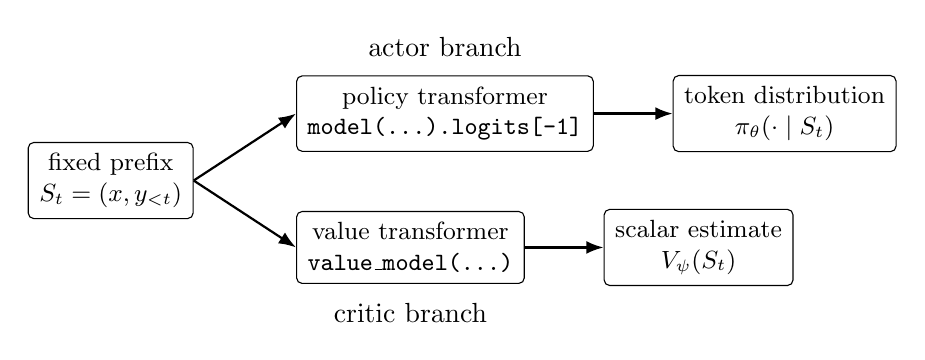
\begin{tikzpicture}[
        node distance=0.9cm and 1.0cm,
        box/.style={draw, rounded corners=2pt, align=center,
                    minimum height=0.9cm, inner sep=4pt, font=\small},
        flow/.style={-{Latex[length=2.2mm]}, thick}
    ]
        \node[box] (state) {fixed prefix\\\(S_t=(x,y_{<t})\)};
        \node[box, right=1.3cm of state, yshift=0.85cm] (policy-model)
            {policy transformer\\\texttt{model(...).logits[-1]}};
        \node[box, right=1.3cm of state, yshift=-0.85cm] (value-model)
            {value transformer\\\texttt{value\_model(...)}};
        \node[box, right=of policy-model] (policy)
            {token distribution\\\(\pi_\theta(\cdot\mid S_t)\)};
        \node[box, right=of value-model] (value)
            {scalar estimate\\\(V_\psi(S_t)\)};

        \draw[flow] (state.east) -- (policy-model.west);
        \draw[flow] (state.east) -- (value-model.west);
        \draw[flow] (policy-model) -- (policy);
        \draw[flow] (value-model) -- (value);

        \node[above=0.12cm of policy-model] {actor branch};
        \node[below=0.12cm of value-model] {critic branch};
    \end{tikzpicture}
    \caption{A separate-model actor--critic implementation.  The policy transformer
    returns the token distribution, and the value transformer returns the
    scalar critic estimate.}
    \label{fig:actor-critic-interface}
\end{figure}

After a rollout, the realized return \(\widehat G_t\) is computed from the
observed rewards after state \(S_t\).  It is one noisy sample of the
conditional mean \(V^\pi(S_t)\).  For a fixed state \(S_t=s\), let \(v\) be a
scalar.  Then

\begin{equation}
    \begin{split}
        \underset{v}{\operatorname{arg\,min}}\;
        \E\left[(v-\widehat G_t)^2\mid S_t=s\right]
        =\E\left[\widehat G_t\mid S_t=s\right]
        =V^\pi(s).
    \end{split}
    \label{eq:value-regression-identity}
\end{equation}

Therefore the critic can be trained by ordinary regression against sampled
returns.  Let \(\widehat{\E}_t\) denote the average over all valid token
positions in the rollout batch.  The critic loss is

\begin{equation}
    \begin{split}
        \mathcal L_V(\psi)
          =\widehat{\E}_t
           \left[\bigl(V_\psi(S_t)-\widehat G_t\bigr)^2\right].
    \end{split}
\end{equation}

For an LLM, one training example for the critic is therefore a prefix
\(S_t=(x,y_{<t})\) paired with the return obtained by its sampled continuation.
The individual return is the comparison target; averaging over many such
examples makes the critic approach the conditional mean.  This is the
auxiliary optimization, not another policy optimization.

The two objectives need not be solved sequentially.  The current critic is
used to compute the advantages for a rollout batch, after which the actor loss
and critic loss are usually optimized together or in alternating minibatch
steps.  The critic improves across rollout batches rather than being solved
exactly before each actor update.

For the response-level reward defined in Section~2, set
\(V_\psi(S_{L+1})=0\) after the response ends.  The residual used by
generalized advantage estimation (GAE) is then\footnote{For general stepwise rewards, the \(\gamma=1\) temporal-difference
residual is \(\delta_t=r_t+V_\psi(S_{t+1})-V_\psi(S_t)\).}

\begin{equation}
    \begin{split}
        \delta_t
        =\begin{cases}
          V_\psi(S_{t+1})-V_\psi(S_t), & 1\leq t<L,\\
          \mathcal R(x,y)-V_\psi(S_L), & t=L.
        \end{cases}
    \end{split}
    \label{eq:llm-td-residual}
\end{equation}

The first line asks whether adding a nonfinal token raises the predicted final
score.  The second line compares the realized response score with the score
predicted before the final token.

More generally, \(r_t+V_\psi(S_{t+1})\) estimates
\(Q^\pi(S_t,a_t)\), and subtracting \(V_\psi(S_t)\) gives an estimated
advantage.  If \(V_\psi=V^\pi\),

\begin{equation}
    \begin{split}
        \E\left[\delta_t\mid S_t,a_t\right]
        &=\E\left[
          r_t+V^\pi(S_{t+1})\mid S_t,a_t
          \right]-V^\pi(S_t)\\
        &=Q^\pi(S_t,a_t)-V^\pi(S_t)\\
        &=A^\pi(S_t,a_t).
    \end{split}
    \label{eq:td-advantage}
\end{equation}

GAE combines the residual at step \(t\) with the residuals at later steps:

\begin{equation}
    \begin{split}
    \widehat A_t^{\mathrm{GAE}}
      =\sum_{\ell=0}^{L-t}
       \lambda^\ell\delta_{t+\ell},
      \qquad 0\leq\lambda\leq1.
    \end{split}
    \label{eq:gae}
\end{equation}

The parameter \(\lambda\) controls how many later residuals matter.  At
\(\lambda=0\), \(\widehat A_t^{\mathrm{GAE}}=\delta_t\).  At \(\lambda=1\),
the sum telescopes to the sampled reward-to-go minus \(V_\psi(S_t)\), assuming
the value after termination is zero.  GAE is one possible advantage estimator;
the clipped update introduced next does not require it.

For fixed sampled paths and fixed advantage estimates \(\widehat A_t\), the
surrogate loss is

\begin{equation}
    \begin{split}
    \mathcal L_{\mathrm{PG}}(\theta)
      =-\widehat{\E}
       \left[
       \sum_{t=1}^{L}
       \widehat A_t
       \log\pi_\theta(a_t\mid S_t)
       \right].
    \end{split}
    \label{eq:policy-gradient-surrogate-expanded}
\end{equation}

Its gradient reproduces the sampled policy-gradient direction at the policy
that generated the paths.

\subsection{Importance sampling and policy reuse}

Let \(\theta_{\mathrm{old}}\) be the model parameters used to generate a
stored batch, and let \(\theta\) be the parameters being optimized.  Define
\(p_\theta(T)=P(T\mid\pi_\theta)\).  The same path \(T\) generally has
different probabilities under \(p_{\theta_{\mathrm{old}}}\) and
\(p_\theta\).  No path variable is transformed, so there is no coordinate
Jacobian.  The change of measure is the likelihood ratio

\begin{equation}
    \begin{split}
    w_t(\theta)
      &\equiv\frac{\pi_\theta(a_t\mid S_t)}
                     {\pi_{\theta_{\mathrm{old}}}(a_t\mid S_t)},\\
    w_\theta(T)
      &\equiv\frac{p_\theta(T)}{p_{\theta_{\mathrm{old}}}(T)}
       =\prod_{t=0}^{N-1}w_t(\theta).
    \end{split}
    \label{eq:path-importance-ratio}
\end{equation}

The initial-state distribution and transition probabilities are the same in
the numerator and denominator of \(w_\theta(T)\), so they cancel.  Only the
policy probabilities remain.  Multiplying by \(w_\theta(T)\) then gives the
exact change of path measure:

\begin{equation}
    \begin{split}
    J(\theta)
      &=\int\mathcal D S\,\mathcal D a\;p_\theta(T)G_0[T]\\
      &=\int\mathcal D S\,\mathcal D a\;p_{\theta_{\mathrm{old}}}(T)
        w_\theta(T)G_0[T]\\
      &=\E_{T\sim p_{\theta_{\mathrm{old}}}}
       \left[
       w_\theta(T)G_0[T]
       \right],
    \end{split}
    \label{eq:importance-objective}
\end{equation}

This permits path reuse, but large ratios make the estimate high-variance.

\newpage
\section{Proximal Policy Optimization}

The motivation for proximal policy optimization (PPO) is computational
efficiency \cite{schulman2017ppo}.  Generating and scoring responses is
expensive; reusing a stored rollout batch for several gradient updates is
cheaper.

Equation~\eqref{eq:importance-objective} already gives the exact
change of measure.  For the current batch, let
\(\pi_{\mathrm{old}}=\pi_{\theta_{\mathrm{old}}}\) be the policy that
generated the responses, and let \(\pi_\theta\) be the policy being updated.
During batch reuse, \(\pi_{\mathrm{old}}\), the sampled states, and the
advantages \(\widehat A_t\) are fixed; only \(\pi_\theta\) changes.  PPO starts
from the token-level conservative policy iteration (CPI) objective

\begin{equation}
    \begin{split}
        J_{\mathrm{CPI}}(\theta)
        =\widehat{\E}_t
         \left[w_t(\theta)\widehat A_t\right],
    \end{split}
    \label{eq:ppo-unclipped-objective}
\end{equation}

where \(w_t(\theta)\) is the likelihood ratio in
Eq.~\eqref{eq:path-importance-ratio}, and \(\widehat{\E}_t\) averages the
valid token positions in the batch.  The advantage is supplied by an
estimator.  The original PPO actor--critic algorithm used
\(\widehat A_t=\widehat A_t^{\mathrm{GAE}}\) from Eq.~\eqref{eq:gae}.

At \(\theta=\theta_{\mathrm{old}}\), Eq.~\eqref{eq:ppo-unclipped-objective}
has the sampled policy-gradient direction.  Repeated updates can move
\(w_t(\theta)\) far from one while the batch remains fixed.  PPO regularizes
Eq.~\eqref{eq:ppo-unclipped-objective} by clipping this favorable change.
For \(\epsilon>0\),
\(\operatorname{clip}(w,a,b)=a\) for \(w<a\), \(b\) for \(w>b\), and \(w\)
otherwise.  The clipped objective is \cite{schulman2017ppo}

\begin{equation}
    \begin{split}
    j_t^{\mathrm{clip}}(\theta)
      &=\begin{cases}
        \widehat A_t\min\!\left(w_t(\theta),1+\epsilon\right),
          & \widehat A_t\geq0,\\
        \widehat A_t\max\!\left(w_t(\theta),1-\epsilon\right),
          & \widehat A_t<0,
        \end{cases}\\
      &=\min\!\left(
          w_t(\theta)\widehat A_t,\,
          \operatorname{clip}
          \bigl(w_t(\theta),1-\epsilon,1+\epsilon\bigr)
          \widehat A_t
       \right),\\
    J_{\mathrm{PPO}}^{\mathrm{clip}}(\theta)
      &=\widehat{\E}_t\left[j_t^{\mathrm{clip}}(\theta)\right].
    \end{split}
    \label{eq:ppo-clipped-objective}
\end{equation}

The piecewise line is the operative rule.  For \(\widehat A_t\geq0\), it
follows \(w_t\widehat A_t\) up to \(w_t=1+\epsilon\); the lower boundary is
inactive.  For \(\widehat A_t<0\), it follows the same term down to
\(w_t=1-\epsilon\); the upper boundary is inactive.  Thus PPO removes the
gradient only after a token ratio has moved too far in the favorable
direction.  It does not hide movement in the unfavorable direction.

The second line is the compact form of the same rule.  It gives
\(j_t^{\mathrm{clip}}\leq w_t\widehat A_t\), a pointwise lower bound on the
sampled contribution, not on the true expected return.  The choice of
\(\epsilon\) controls how far the batch is reused; clipping is not a
convergence guarantee \cite{wang2020trulyppo}.

The reference policy \(\pi_{\mathrm{ref}}\) is different from
\(\pi_{\mathrm{old}}\).  It is usually the initial supervised model and
remains fixed throughout training.  Let \(c_V\geq0\) weight the critic loss
and let \(\beta\geq0\) weight the optional Kullback--Leibler (KL) penalty to
\(\pi_{\mathrm{ref}}\).  The combined LLM training loss is
\cite{schulman2017ppo,ouyang2022instructgpt}

\begin{equation}
    \begin{split}
    \mathcal L_{\mathrm{PPO}}(\theta,\psi)
      =-J_{\mathrm{PPO}}^{\mathrm{clip}}(\theta)
       +c_V\,\widehat{\E}_t
        \left[
          \bigl(V_\psi(S_t)-\widehat G_t\bigr)^2
        \right]
       +\beta\,\widehat{\E}_t
        \left[
          \KL\!\left(
          \pi_\theta(\cdot\mid S_t)
          \,\|\,\pi_{\mathrm{ref}}(\cdot\mid S_t)
          \right)
        \right].
    \end{split}
    \label{eq:ppo-total-loss}
\end{equation}

Equation~\eqref{eq:ppo-total-loss} is minimized.  Its three terms update the
policy, fit the value emulator to the single target \(\widehat G_t\), and
limit cumulative drift from the reference policy, respectively.

PPO is a battle-tested LLM post-training baseline.  InstructGPT used PPO with
a separate value function and one inner epoch per rollout batch
\cite{ouyang2022instructgpt}.  NVIDIA's current NeMo RL stack describes PPO as
widely used and supports it at production scale \cite{nvidia2026ppo}.  Its PPO
recipe is nevertheless much larger than Eq.~\eqref{eq:ppo-clipped-objective}:
it includes a value model, optional critic warm-up, independent actor and
critic update counts, KL control, and critic and policy diagnostics.  Thus
production PPO is rarely just the clipped objective from the original paper.

The practical limitation of vanilla PPO is not the likelihood ratio itself.
The ratio is the correct local change-of-measure factor.  The difficulty is
the collection of approximations around it: finite rollout batches, fixed
advantages during batch reuse, token-level rather than complete-path ratios,
a learned critic, and clipping.  The critic adds memory and optimization cost
and can introduce value bias.  Ratio clipping does not enforce a strict trust
region \cite{wang2020trulyppo}.  For long responses with sparse terminal
rewards, value bias and decay of the propagated reward signal can become
important \cite{yuan2025ppocollapse}.

This cost motivated critic-free alternatives.  A study of ordinary RLHF found
that simpler REINFORCE-style estimators could outperform PPO while requiring
less computation \cite{ahmadian2024backtobasics}.  DeepSeekMath introduced
group-relative policy optimization (GRPO) specifically to remove PPO's value
model \cite{shao2024deepseekmath}, and DeepSeek-R1 subsequently used GRPO in
its reasoning-training pipeline
\cite{deepseekai2025r1}.

Removing the critic does not settle the stability problem.  In the DAPO
experiments, a naive GRPO run exhibited entropy collapse, reward noise, and
training instability.  DAPO added asymmetric clipping, dynamic sampling,
token-level loss aggregation, and overlong-response shaping
\cite{yu2025dapo}.  Qwen's later group sequence policy optimization (GSPO)
replaced token-level importance ratios and clipping by sequence-level versions
and reported improved stability relative to GRPO, particularly for
mixture-of-experts training \cite{zheng2025gspo}.  These are reported results
of the respective systems, not a universal ranking of the objectives.

The development has also moved back toward value-based methods.  VAPO retains
a critic but changes its initialization, targets, and advantage construction
for long reasoning traces \cite{yue2025vapo}.  Its motivation is that a
well-trained critic can provide token-level credit assignment that a single
response score cannot, while the preceding failure analysis shows why an
ordinary critic may fail \cite{yuan2025ppocollapse}.  The resulting practical
picture is therefore conditional: vanilla PPO is established but
high-maintenance; a carefully trained critic may help long-horizon credit
assignment; and GRPO is cheaper when several responses can be scored directly.
Direct preference optimization (DPO) addresses a different regime in which
training uses a fixed preference dataset rather than new online responses.

GRPO keeps online generation, the old-policy likelihood ratio, and a PPO-style
clipped actor update, but replaces the value emulator by a comparison among
several complete responses to the same prompt.

\newpage
\section{Group-Relative Policy Optimization}

\subsection{Group-relative advantage}

For one prompt \(x\), let \(K\geq2\) be the number of complete responses
sampled from the frozen policy \(\pi_{\mathrm{old}}\), let
\(k=1,\ldots,K\) index a response, and let \(L_k\) be its length:

\begin{equation}
    \begin{split}
    y^{(k)}&\sim\pi_{\mathrm{old}}(\cdot\mid x),\\
    \mathcal R_k&=\mathcal R(x,y^{(k)}).
    \end{split}
    \label{eq:grpo-rollouts}
\end{equation}

GRPO does not estimate \(V^\pi\).  It instead compares the \(K\) scores for
the same prompt.  With a numerical stabilizer \(\varepsilon_R>0\), the
supplied implementation uses the sample standard deviation:

\begin{equation}
    \begin{split}
    \overline{\mathcal R}
      &=\frac{1}{K}\sum_{j=1}^{K}\mathcal R_j,\\
    s_{\mathcal R}
      &=\sqrt{\frac{1}{K-1}
        \sum_{j=1}^{K}(\mathcal R_j-\overline{\mathcal R})^2},\\
    \widehat A_k^{\mathrm{GRPO}}
      &=\frac{\mathcal R_k-\overline{\mathcal R}}
              {s_{\mathcal R}+\varepsilon_R}.
    \end{split}
    \label{eq:grpo-advantage}
\end{equation}

\subsection{The token-level clipped objective}

For response \(k\), define \(S_t^{(k)}=(x,y_{<t}^{(k)})\).  The probability
ratio for token \(y_t^{(k)}\) is

\begin{equation}
    \begin{split}
    w_{kt}(\theta)
      =\frac{
        \pi_\theta(y_t^{(k)}\mid S_t^{(k)})
      }{
        \pi_{\mathrm{old}}(y_t^{(k)}\mid S_t^{(k)})
      }.
    \end{split}
    \label{eq:grpo-token-ratio}
\end{equation}

The same response-level advantage \(\widehat A_k^{\mathrm{GRPO}}\) weights
every token in that response.  GRPO maximizes the length-normalized objective

\begin{equation}
    \begin{split}
    J_{\mathrm{GRPO}}^{\mathrm{clip}}(\theta)
      =\frac{1}{K}\sum_{k=1}^{K}\frac{1}{L_k}
       \sum_{t=1}^{L_k}
       \min\!\Bigl(
          w_{kt}(\theta)\widehat A_k^{\mathrm{GRPO}},\,
          \operatorname{clip}
          \bigl(w_{kt}(\theta),1-\epsilon,1+\epsilon\bigr)
          \widehat A_k^{\mathrm{GRPO}}
       \Bigr).
    \end{split}
    \label{eq:grpo-clipped-objective}
\end{equation}

The supplied implementation also compares the current policy with the fixed
reference policy.  For the sampled token \(y_t^{(k)}\), let
\(p_{kt}=\pi_\theta(y_t^{(k)}\mid S_t^{(k)})\) and
\(q_{kt}=\pi_{\mathrm{ref}}(y_t^{(k)}\mid S_t^{(k)})\).  The sampled KL
penalty is
\(\widehat D_{kt}=q_{kt}/p_{kt}-\log(q_{kt}/p_{kt})-1\geq0\)
\cite{shao2024deepseekmath}.  Its conditional expectation over
\(y_t^{(k)}\sim\pi_\theta(\cdot\mid S_t^{(k)})\) is
\(\KL\!\left(\pi_\theta(\cdot\mid S_t^{(k)})\,\|\,
\pi_{\mathrm{ref}}(\cdot\mid S_t^{(k)})\right)\).\footnote{For \(z>0\),
\(z-\log z-1\geq0\).  \textcolor{red}{At fixed \(S_t^{(k)}\), write
\(p(y)=\pi_\theta(y\mid S_t^{(k)})\) and
\(q(y)=\pi_{\mathrm{ref}}(y\mid S_t^{(k)})\).  Since \(q\) is normalized,
\(\E_{y\sim p}[q(y)/p(y)]
=\sum_y p(y)q(y)/p(y)=\sum_y q(y)=1\).  Therefore
\(\E_{y\sim p}[q(y)/p(y)-1]=0\).}}

During later reuse of the same batch, its tokens come from
\(\pi_{\mathrm{old}}\), not exactly from \(\pi_\theta\).  The expectation
identity in the footnote then no longer holds exactly for the stored batch, so
its mean is only a local estimate of the current-policy KL.

Let \(\beta\geq0\) control this penalty.  The complete loss minimized by the
implementation is

\begin{equation}
    \begin{split}
    \mathcal L_{\mathrm{GRPO}}(\theta)
      &=-J_{\mathrm{GRPO}}^{\mathrm{clip}}(\theta)\\
      &\quad+\frac{\beta}{K}\sum_{k=1}^{K}\frac{1}{L_k}
       \sum_{t=1}^{L_k}\widehat D_{kt}.
    \end{split}
    \label{eq:grpo-total-loss}
\end{equation}

Thus GRPO changes the source of the advantage estimate; its actor update is
still PPO-style.  The three methods differ in the weight multiplying
\(\nabla_\theta\log\pi_\theta\):

\begin{equation}
    \begin{split}
    \text{REINFORCE:}\quad
      \widehat A_k&=\mathcal R_k,\\
    \text{PPO with critic:}\quad
      \widehat A_t&=\widehat A_t^{\mathrm{GAE}},\\
    \text{GRPO:}\quad
      \widehat A_k&=\frac{\mathcal R_k-\overline{\mathcal R}}
                          {s_{\mathcal R}+\varepsilon_R}.
    \end{split}
    \label{eq:advantage-family}
\end{equation}

\newpage
\section{Online and Offline Training}

Equation~\eqref{eq:expected-return} averages over all possible paths.  In
practice, we replace this path integral by an average over a finite batch.
Let \(n\) label an optimization step, let \(M\) be the number of paths in its
batch, and let \(m=1,\ldots,M\) index a path.  Write

\begin{equation}
    \begin{split}
    \mathcal B_n
    &=\{T_n^{(1)},\ldots,T_n^{(M)}\},\\
    T_n^{(m)}&\sim q_n(T).
    \end{split}
    \label{eq:sampling-measure}
\end{equation}

Here \(\mathcal B_n\) is the batch and \(q_n(T)\) is the probability
distribution from which its paths are drawn.  The subscript \(n\) allows this
distribution to change during training.  Let \(F(T)\) be any quantity
computed from a path, such as its return or its loss.  Its expectation is
estimated by

\begin{equation}
    \begin{split}
        \widehat{\E}_{q_n}[F]
        =\frac{1}{M}\sum_{m=1}^{M}F(T_n^{(m)}).
    \end{split}
    \label{eq:batch-average}
\end{equation}

This is the finite-batch version of the path integral.  To distinguish offline
and online training, define \(q_{\mathrm{data}}(T)\) as the distribution of
paths in a fixed dataset, and define
\(p_{\theta_n}(T)=P(T\mid\pi_{\theta_n})\) as the path distribution
generated by the policy at step \(n\).  Then

\begin{equation}
    \begin{split}
    \text{offline:}\quad q_n(T)&=q_{\mathrm{data}}(T),\\
    \text{online:}\quad q_n(T)&=p_{\theta_n}(T).
    \end{split}
    \label{eq:offline-online}
\end{equation}

Offline training samples stored paths from \(q_{\mathrm{data}}\), which does
not change when the model changes.  Online training samples new paths from
\(p_{\theta_n}\), so changing the model changes the paths available for later
updates.

The same distinction appears in the objectives.  Let \(\Xi\) denote one
stored training record: a single supervised response, or a pair of response
paths with their preference label.  Let \(q_{\mathrm{data}}(\Xi)\) be the
fixed distribution of these records, and let \(\ell_\theta(\Xi)\) be the loss
assigned to one record.  Then

\begin{equation}
    \begin{split}
    \mathcal L_{\mathrm{off}}(\theta)
      &=\E_{\Xi\sim q_{\mathrm{data}}}
        \left[\ell_\theta(\Xi)\right],\\
    J(\theta)
      &=\E_{T\sim p_\theta}\left[G_0[T]\right].
    \end{split}
    \label{eq:offline-online-objectives}
\end{equation}

In the offline objective, \(\theta\) changes the loss but not the stored
records.  In the online objective, \(G_0[T]\) is the complete-path return from
Eq.~\eqref{eq:return}, and \(\theta\) changes the path distribution
\(p_\theta(T)\).  Supervised fine-tuning and DPO use the first form; PPO and
GRPO use the second.

For LLM training, \emph{online} means that responses are generated during
training.  A batch is \emph{on-policy} only for the policy that generated it.
After that policy is updated, reuse of the batch requires the likelihood ratio
in Eq.~\eqref{eq:path-importance-ratio}.

\subsection{Supervised fine-tuning}

Let \(q_{\mathrm{SFT}}(x,y)\) be the empirical distribution of a fixed
prompt--response dataset.  Supervised fine-tuning (SFT) minimizes

\begin{equation}
    \begin{split}
    \mathcal L_{\mathrm{SFT}}(\theta)
      &=-\E_{(x,y)\sim q_{\mathrm{SFT}}}
        \left[\log\pi_\theta(y\mid x)\right]\\
      &=-\E_{(x,y)\sim q_{\mathrm{SFT}}}
        \left[\sum_{t=1}^{L}
        \log\pi_\theta(y_t\mid x,y_{<t})\right].
    \end{split}
    \label{eq:sft}
\end{equation}

This increases the probability of the demonstrated paths.

\subsection{Preference data and reward modeling}

Let \(q_{\mathrm{pref}}(x,y^+,y^-)\) be a fixed dataset of preference triples:
a prompt \(x\), a preferred response \(y^+\), and a rejected response \(y^-\).
A scalar reward model \(\mathcal R_\phi\), with parameters \(\phi\), defines

\begin{equation}
    \begin{split}
    P_\phi(y^+\succ y^-\mid x)
      =\sigma\!\left(
        \mathcal R_\phi(x,y^+)-\mathcal R_\phi(x,y^-)
      \right),
    \end{split}
    \label{eq:preference-probability}
\end{equation}

where \(\sigma(z)=1/(1+e^{-z})\) is the logistic sigmoid.  Thus
\(P_\phi\) is the model's probability that \(y^+\) is preferred to \(y^-\).

The reward-model loss is

\begin{equation}
    \begin{split}
    \mathcal L_{\mathrm{RM}}(\phi)
      =-\E_{(x,y^+,y^-)\sim q_{\mathrm{pref}}}
       \log P_\phi(y^+\succ y^-\mid x).
    \end{split}
    \label{eq:reward-model-loss}
\end{equation}

This is not a policy-gradient loss.  The preference dataset is fixed, the
optimized parameters are \(\phi\), and the logarithm acts on the predicted
preference probability.  The result is a reward model that assigns scalar
scores to complete responses.

\subsection{Direct Preference Optimization}

For a prompt \(x\) and complete response \(y\), let \(\mathcal R(x,y)\) be
the sequence score defined in Section~2.  The derivation uses this score to
connect the online objective to preference probabilities; DPO training will
eliminate it from the loss.  Let \(\pi_{\mathrm{ref}}(y\mid x)\) be a fixed
reference LLM, and let \(\beta>0\) control the penalty for moving away from
that reference.  To derive the optimum, first treat
\(\pi(y\mid x)\) as any normalized conditional distribution over complete
responses.  The trainable LLM \(\pi_\theta\) will be substituted afterward.
The KL-regularized objective is \cite{rafailov2023dpo}

\begin{equation}
    \begin{split}
    J_\beta(\pi)
      =\E_{x\sim q}\!\left[
        \sum_y\pi(y\mid x)
        \left(
        \mathcal R(x,y)
        -\beta\log\frac{\pi(y\mid x)}
                            {\pi_{\mathrm{ref}}(y\mid x)}
        \right)
      \right].
    \end{split}
    \label{eq:kl-regularized-objective}
\end{equation}

Equation~\eqref{eq:kl-regularized-objective} is maximized; it is not a loss to
be minimized.  If \(\pi\) moves farther from \(\pi_{\mathrm{ref}}\), the KL
divergence grows and the subtraction makes \(J_\beta\) smaller.  Equivalently,
one may minimize

\begin{equation}
    \begin{split}
    \mathcal L_\beta(\pi)
    &=-J_\beta(\pi)\\
    &=-\E_{x\sim q,\,y\sim\pi(\cdot\mid x)}
       \left[\mathcal R(x,y)\right]
      +\beta\E_{x\sim q}
       \KL\!\left(
       \pi(\cdot\mid x)\,\|\,\pi_{\mathrm{ref}}(\cdot\mid x)
       \right).
    \end{split}
    \label{eq:kl-regularized-loss}
\end{equation}

In the loss, moving away makes the positive KL term larger.  Larger \(\beta\)
therefore keeps the policy closer to the reference; smaller \(\beta\) lets the
reward dominate.

Equation~\eqref{eq:kl-regularized-loss} is the loss for online RL with an
explicit reward \(\mathcal R(x,y)\).  It is not the DPO loss.  Optimizing it
requires sampling responses from \(\pi\) and evaluating their rewards.  DPO
instead uses fixed preference triples \((x,y^+,y^-)\) and optimizes the
pairwise loss below.  The two losses are not added together.

For each fixed prompt, maximizing Eq.~\eqref{eq:kl-regularized-objective}
over normalized response distributions gives

\begin{equation}
    \begin{split}
    Z(x)
      &=\sum_y\pi_{\mathrm{ref}}(y\mid x)
        \exp\!\left(\frac{\mathcal R(x,y)}{\beta}\right),\\
    \pi^*(y\mid x)
      &=\frac{\pi_{\mathrm{ref}}(y\mid x)}{Z(x)}
        \exp\!\left(\frac{\mathcal R(x,y)}{\beta}\right),\\
    \mathcal R(x,y)
      &=\beta\log
        \frac{\pi^*(y\mid x)}{\pi_{\mathrm{ref}}(y\mid x)}
        +\beta\log Z(x),\\
    \mathcal R(x,y^+)-\mathcal R(x,y^-)
      &=\beta\left[
        \log\frac{\pi^*(y^+\mid x)}{\pi_{\mathrm{ref}}(y^+\mid x)}
        -\log\frac{\pi^*(y^-\mid x)}{\pi_{\mathrm{ref}}(y^-\mid x)}
        \right].
    \end{split}
    \label{eq:dpo-policy-reward}
\end{equation}

The factor \(Z(x)\) enforces \(\sum_y\pi^*(y\mid x)=1\).  It is constant when
two responses to the same prompt are compared, so it cancels in the last line.
DPO substitutes that reward difference into
Eq.~\eqref{eq:preference-probability} and replaces \(\pi^*\) by the trainable
policy \(\pi_\theta\).  The resulting loss is

\begin{equation}
    \begin{split}
    \mathcal L_{\mathrm{DPO}}(\theta)
      =-\E_{(x,y^+,y^-)\sim q_{\mathrm{pref}}}
      \log\sigma\!\Bigg(
      \beta\Bigg[
      &\log\frac{\pi_\theta(y^+\mid x)}
                     {\pi_{\mathrm{ref}}(y^+\mid x)}
      -
      \log\frac{\pi_\theta(y^-\mid x)}
                     {\pi_{\mathrm{ref}}(y^-\mid x)}
      \Bigg]\Bigg).
    \end{split}
    \label{eq:dpo-loss}
\end{equation}

This loss is minimized over \(\theta\); \(\beta\), \(\pi_{\mathrm{ref}}\), and
the preference triples are fixed.  Its bracket is the preferred response's
log-probability change relative to the reference minus the corresponding
change for the rejected response.  DPO therefore needs no explicit reward
evaluation or on-policy response generation during an update.

The methods discussed in the note can now be compared without introducing
any new objects:

\begin{center}
\small
\begin{tabularx}{\textwidth}{@{}l Y Y Y Y@{}}
\toprule
Method & Paths used & Quantity optimized & Critic & Additional policy \\
\midrule
SFT
& Demonstrations from \(q_{\mathrm{SFT}}\)
& Demonstration log-likelihood
& No
& None \\
DPO
& Preference pairs from \(q_{\mathrm{pref}}\)
& Pairwise policy log-ratio
& No
& \(\pi_{\mathrm{ref}}\) \\
REINFORCE
& Responses sampled from \(\pi_\theta\)
& \(G_t\log\pi_\theta(a_t\mid S_t)\)
& No
& None \\
PPO
& Responses sampled from \(\pi_{\mathrm{old}}\)
& Clipped \(w_t\widehat A_t\)
& Optional; used with GAE
& \(\pi_{\mathrm{old}}\) per batch; optional \(\pi_{\mathrm{ref}}\) \\
GRPO
& \(K\) responses per prompt from \(\pi_{\mathrm{old}}\)
& Clipped \(w_{kt}\widehat A_k^{\mathrm{GRPO}}\)
& No
& \(\pi_{\mathrm{old}}\) per batch; optional \(\pi_{\mathrm{ref}}\) \\
\bottomrule
\end{tabularx}
\end{center}

\newpage
\begin{thebibliography}{99}

\bibitem{schulman2017ppo}
J.~Schulman, F.~Wolski, P.~Dhariwal, A.~Radford, and O.~Klimov,
\emph{Proximal Policy Optimization Algorithms}, 2017.
\url{https://arxiv.org/abs/1707.06347}.

\bibitem{ouyang2022instructgpt}
L.~Ouyang et al.,
\emph{Training Language Models to Follow Instructions with Human Feedback},
NeurIPS 2022.
\url{https://arxiv.org/abs/2203.02155}.

\bibitem{rafailov2023dpo}
R.~Rafailov, A.~Sharma, E.~Mitchell, S.~Ermon, C.~D.~Manning, and C.~Finn,
\emph{Direct Preference Optimization: Your Language Model Is Secretly a
Reward Model}, NeurIPS 2023.
\url{https://arxiv.org/abs/2305.18290}.

\bibitem{wang2020trulyppo}
Y.~Wang, H.~He, and X.~Tan,
\emph{Truly Proximal Policy Optimization},
Proceedings of Machine Learning Research 115, 113--122, 2020.
\url{https://proceedings.mlr.press/v115/wang20b.html}.

\bibitem{ahmadian2024backtobasics}
A.~Ahmadian, C.~Cremer, M.~Gall\'e, M.~Fadaee, J.~Kreutzer,
O.~Pietquin, A.~\"Ust\"un, and S.~Hooker,
\emph{Back to Basics: Revisiting REINFORCE Style Optimization for Learning
from Human Feedback in LLMs}, 2024.
\url{https://arxiv.org/abs/2402.14740}.

\bibitem{shao2024deepseekmath}
Z.~Shao et al.,
\emph{DeepSeekMath: Pushing the Limits of Mathematical Reasoning in Open
Language Models}, 2024.
\url{https://arxiv.org/abs/2402.03300}.

\bibitem{deepseekai2025r1}
DeepSeek-AI,
\emph{DeepSeek-R1: Incentivizing Reasoning Capability in LLMs via
Reinforcement Learning}, 2025.
\url{https://arxiv.org/abs/2501.12948}.

\bibitem{yu2025dapo}
Q.~Yu et al.,
\emph{DAPO: An Open-Source LLM Reinforcement Learning System at Scale}, 2025.
\url{https://arxiv.org/abs/2503.14476}.

\bibitem{zheng2025gspo}
C.~Zheng et al.,
\emph{Group Sequence Policy Optimization}, 2025.
\url{https://arxiv.org/abs/2507.18071}.

\bibitem{yuan2025ppocollapse}
Y.~Yuan, Y.~Yue, R.~Zhu, T.~Fan, and L.~Yan,
\emph{What's Behind PPO's Collapse in Long-CoT? Value Optimization Holds the
Secret}, 2025.
\url{https://arxiv.org/abs/2503.01491}.

\bibitem{yue2025vapo}
Y.~Yue et al.,
\emph{VAPO: Efficient and Reliable Reinforcement Learning for Advanced
Reasoning Tasks}, 2025.
\url{https://arxiv.org/abs/2504.05118}.

\bibitem{nvidia2026ppo}
NVIDIA,
\emph{An In-Depth Walkthrough of PPO in NeMo RL}, accessed September 5, 2026.
\url{https://docs.nvidia.com/nemo/rl/nightly/guides/ppo.html}.

\end{thebibliography}

\end{document}
